
\section*{Ejercicio 2}
\subsection{Análisis teórico}
El circuito a analiza consiste, a grandes rasgos, en un amplificador no inversor.
Para su estudio teórico se tomarán dos modelos, donde, en primer lugar, se considerará al amplificador operacional en su versión ideal, para luego introducir no idealidades en su impedancia de entrada, salida y en la ganancia del mismo.
Los valores de las resistencias a utilizar fueron reemplazados por su valor comercial más cercano, resultando en que el circuito a analizar sea el de la figura \ref{fig: Initial circuit}
\begin{figure}[H]
    \begin{minipage}{\textwidth}
        \centering
        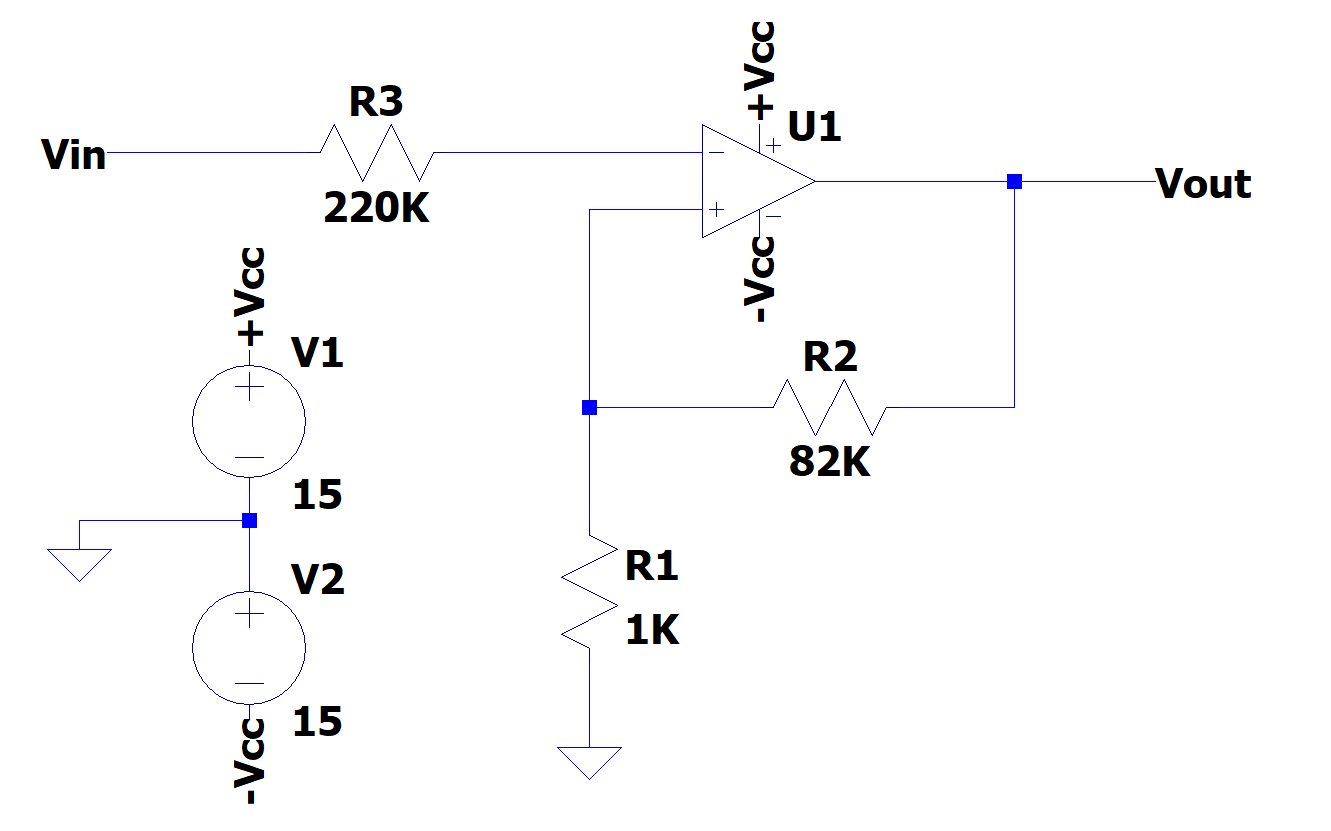
\includegraphics[width=\textwidth]{../EJ2/recursos_para_el_informe/circuito_a_analizar}
        \caption{Circuito a analizar.}
        \label{fig: Initial circuit}
    \end{minipage}\hfill
\end{figure}


\subsubsection{Modelo ideal}
La primer aproximación al comportamiento del circuito se realizará considerando al amplificador operacional como un componente ideal, es decir, $Av = \inf$, $Z_{in_{opamp}} = \inf$, $Z_{out_{opamp}} = 0$.
De esta manera, sin importar el modelo de operacional utilizado, se tiene que:
\begin{equation}
    \label{eq: Ideal Gain}
    \frac{v_{out}}{v_{in}} = 1 + \frac{R_2}{R_1} = 1 + \frac{82 K\Omega}{1 K\Omega} = 83 \implies 38,38 dB
\end{equation}

Se desprende también, de las condiciones de idealidad impuestas, que la impedancia de entrada del circuito será infinita.


\subsubsection{Modelo con impedancia de entrada, salida, y ganancia finita}
Para la resolución del circuito con las consideraciones ya mencionadas, es necesario ahora especificar qué datos serán utilizados para los cálculos.
Los mismos se presentan en la tabla
\begin{table}[]
    \label{tab: Parameters for equations}
    \begin{tabular}{|l|llllll|}
        \hline
        \textbf{\begin{tabular}[c]{@{}l@{}}Modelo de \\ operacional\end{tabular}} & \textbf{\begin{tabular}[c]{@{}l@{}}$f_0$ según \\ datasheet (Hz)\end{tabular}} & \textbf{\begin{tabular}[c]{@{}l@{}}$f_0$ según modelo\\ de spice (Hz)\end{tabular}} & \textbf{\begin{tabular}[c]{@{}l@{}}$A_0$ según \\ datasheet\end{tabular}} & \textbf{\begin{tabular}[c]{@{}l@{}}$A_0$ según\\ modelo de spice\end{tabular}} & \textbf{$Z_{in_{opamp}}(K\Omega)$} & \textbf{$Z_{out_{opamp}}(\Omega)$} \\ \hline
        \textbf{LM833}                                                            & $16 \cdot 10^3$                                                                          & $143,1$                                                                               & $1000$                                                                      & $10 \cdot 10^5$                                                                          & $175$                                  & $37$                                   \\
        \textbf{NE5534}                                                           & $100 \cdot 10^3$                                                                         & $13,88 \cdot 10^6$                                                                            & $10 \cdot 10^5$                                                                     & $10 \cdot 10^5$                                                                          & $100$                                  & $0,3$                                  \\ \hline
        \end{tabular}
    \caption{Tabla de parámetros para cálculo de circuito no ideal.}
\end{table}

